Din punctul de vedere al unui dezvoltator software am observat in timpul experientei faptul ca pentru echipa efectiva de dezvoltare era destul de dificil de intretinut baza de date (ma refer chiar si la pornit/oprit, mai ales pentru juniori acest lucru putea pune probleme daca baza de date se afla instalata pe o platforma UNIX). In cazul in care se dorea aplicarea unei strategii de point in time recovery pentru restabilirea bazei de date la o stare existenta la un moment dat, era nevoie de interventia echipei de devOps, ceea ce se factura diferit la client, prin urmare trebuia convins in prealabil Product Owner-ul de necesitatea acelei interventii si planificat totul.
\par
Astfel ca, am observat necesitatea existentei unei aplicatii care sa usureze operatiile asupra bazei de date, incepand cu pornirea/oprirea/verificarea statusului pana la intreaga operatie de backup si point in time recovery(intoarcere la o stare existenta la un anumit moment dat). Aceasta aplicatie trebuia sa fie intuitiva, usor de folosit chiar si pentru cineva care nu avea cunostinte de devOps, nefiind necesar accesul efectiv pe masina de UNIX unde se afla clusterul de baze de date. Este de la sine inteles ca aplicatia ar trebui sa detecteze toate bazele de date din clusterul de pe masina pe care este incarcata si ar trebui sa permita operatiile prezentate mai sus pentru fiecare dintre instanta in parte.
\section{Arhitectura sistemului de fisiere}
Am propus o solutie pentru bazele de date PostgreSQL folosite pe platforme UNIX (la momentul de fata). Pentru a prezenta solutia software am avut nevoie de un mediu UNIX pe care sa ruleze un numar de instante PostgreSQL. Am ales o masina CentOS, instanta EC2 oferita de Amazon. Sistemul de fisiere a fost organizat folosind LVM (logical volume manager) dupa cum urmeaza:
\begin{itemize}
\item am cerut 3 discuri de cate 50GiB, Amazon EBS;
\item am creat cate un physical volume din fiecare din cele 3 discuri;
\item am creat un volume group si le-am adaugat acestuia;
\item am creat 6 logical volumes, 3 seturi de cate 2 logical volumes; un logical volume de 20GiB pentru datele din db si un logical volume de 10GiB pentru stocarea fisierelor WAL.
\end{itemize}
Au mai ramas 60GiB nealocati, acestia putand fi folositi ulterior. Daca se observa ca un client are nevoie de mai mult spatiu i se pot extinde logical volumes folosind din spatiul nealocat, acesta fiind mare avantaj al LVM. Bazele de date nu vor fi intrerupte cat timp se face extinderea logical volumes.
\par
Am setat astfel sistemul de fisiere pentru 3 instante diferite de baze de date PostgreSQL denumite lv-pgdata-1, lv-pgdata-2 si lv-pgdata-3. In \textit{Figura 1} este prezentata diagrama sistemului de fisiere.
\begin{figure}[h]
	\centering
	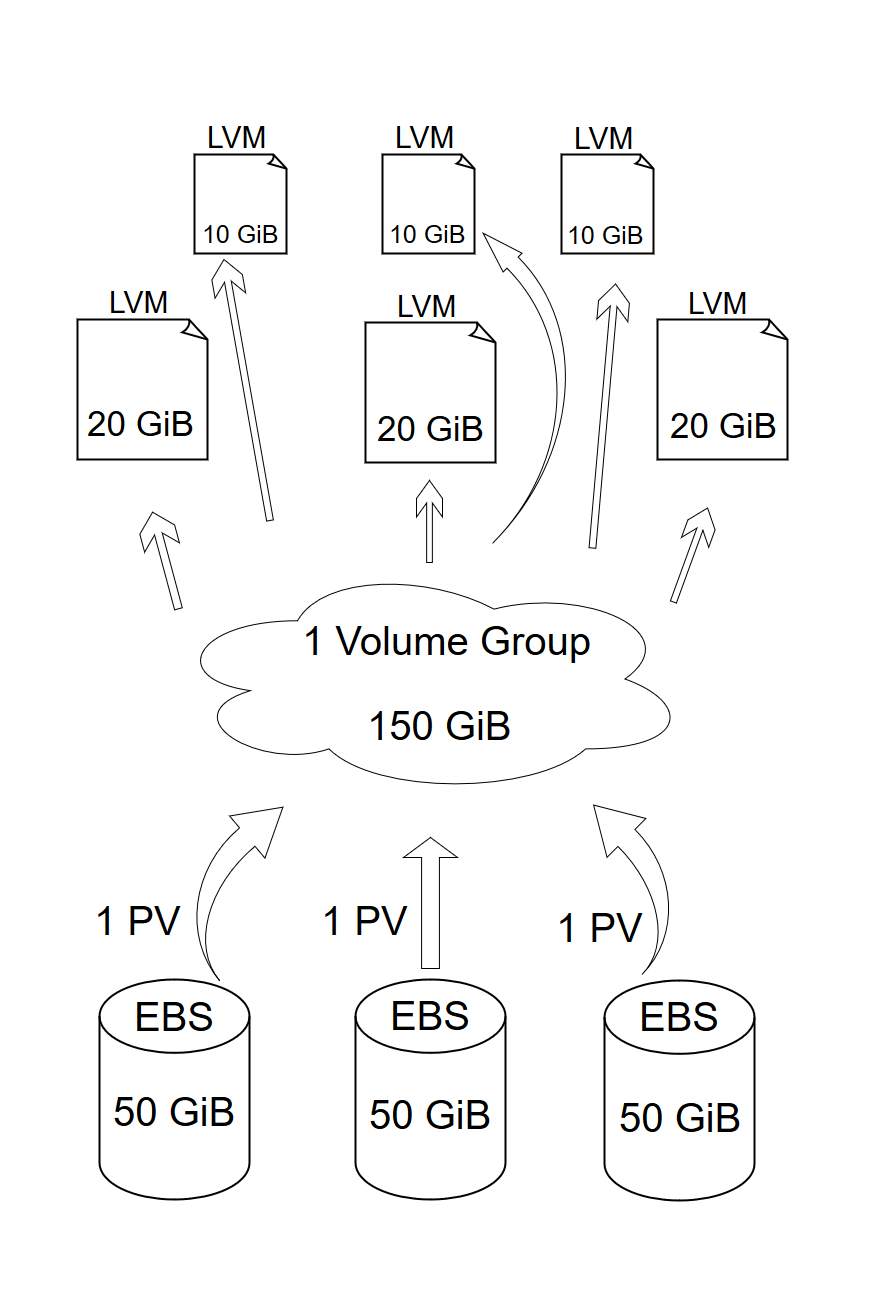
\includegraphics[scale=0.555]{LVM}
    \caption{Diagrama sistemului de fisiere}
    \label{fig:diagSistFiles}
\end{figure}